\chapter{Implementation}
To measure the performance of various data structures, we implemented them
in the C programming language (using the C11 revision).
We have chosen this language for several reasons:
\begin{itemize}
\item The language is low-level, which enables a high degree of tuning by hand.
	Our data structures are also not slowed down by common features of
	high-level languages, such as garbage collection.
\item C toolchains are mature and they can be expected to optimize code well.
\item The C language is very portable and most other languages can
	call C functions. This enables our data structures to be potentially
	easily used in other projects.
\end{itemize}

Our code was developed using the GNU C Compiler (version 4.9.2) on Linux.
We used the Git version control system, with our repository hosted at
\url{https://github.com/MichalPokorny/thesis}. The code includes a test suite,
which tests implementation details of particular data structures as well
as general fuzz tests for checking that implemented data structures behave
like proper dictionaries. We used Travis CI (\url{https://travis-ci.org/})
to automatically test our code after submission.

All dictionaries assume 64-bit keys and values (represented as the
\texttt{uint64\_t} type). It would be easy to allow keys and values of arbitrary
size, but such a choice would be likely to slow down operations on
the data structures, because a range of compiler optimizations would
be impossible in code assuming general lengths. For example, copying
keys and values would need to be a general loop or
\texttt{memcpy}/\texttt{memmove} call, while assuming a constant key/value
size of 64 bits lets us copy in one CPU instruction. Using the C++ language,
we could potentially use templates to make our data structures both general
and optimized. If we are willing to sacrifice some code style, we could
make the C code behave similarly by moving the implementation into a header
file, which could be configured to generate a general data structure
tuned to specific parameters prior to inclusion, as in the following example:
\begin{lstlisting}
struct my_value {
	uint64_t stuff[32];
};
#define IMPLEMENTATION_PREFIX myimpl
#define IMPLEMENTATION_KEY_TYPE uint64_t
#define IMPLEMENTATION_VALUE_TYPE struct my_value
#include "btree/general.impl.h"

void usage() {
	dict* btree;
	dict_init(&btree, &dict_myimpl_btree);
	// ...
}
\end{lstlisting}
For example, the LibUCW library (\url{http://www.ucw.cz/libucw/})
uses this pattern for generic hash tables. We have decided to forgo generality
to keep the code clean and readable.

\section{General dictionary API}
All implemented data structures can be used through a common API defined
in \texttt{dict/dict.h}. To encapsulate implementation details from
users of the API, we have used a common C "trick", where we represent
dictionaries as "virtual table pointers" and "private data".
The common API represents a dictionary as a pointer to an opaque structure.
The type pointed to is declared in \texttt{dict/dict.h} as:
\begin{lstlisting}[language=C]
typedef struct dict_s dict;
\end{lstlisting}

The \texttt{struct dict\_s} structure is defined in \texttt{dict/dict.c}
to prevent exposure of implementation details from users including
\texttt{dict/dict.h}:
\begin{lstlisting}[language=C]
struct dict_s {
	void* opaque;
	const dict_api* api;
};
\end{lstlisting}

The \texttt{opaque} pointer is maintained by the concrete implementation.
\texttt{dict\_api} is a "virtual method table" type defined in
\texttt{dict/dict.h}:

\begin{lstlisting}[language=C]
typedef struct {
	int8_t (*init)(void**);
	void (*destroy)(void**);

	int8_t (*find)(void*, uint64_t key,
			uint64_t *value, bool *found);
	int8_t (*insert)(void*, uint64_t key, uint64_t value);
	int8_t (*delete)(void*, uint64_t key);

	const char* name;

	// More function pointers.
} dict_api;
\end{lstlisting}

The \texttt{init} and \texttt{destroy} functions are passed a pointer to the
\texttt{opaque} pointer and they respecively initialize and deinitialize it.
The \texttt{name} field is a human-readable name of the data structure.
Other fields are given the \texttt{opaque} pointer as the first argument
and they act as implementations of their respective general versions operating
on general dictionaries declared in \texttt{dict/dict.h}:

\begin{lstlisting}[language=C]
void dict_find(dict*, uint64_t key,
		uint64_t *value, bool *found);
int8_t dict_insert(dict*, uint64_t key, uint64_t value);
int8_t dict_delete(dict*, uint64_t key);
\end{lstlisting}

Dictionary data structures may optionally implement successor and predecessor
lookups. The public API consists of the functions \texttt{dict\_next} and
\texttt{dict\_prev}. If the data structure does not implement these operations,
it may set the appropriate fields in \texttt{dict\_api} to \texttt{NULL}.
The \texttt{dict\_api\_allows\_order\_queries} and
\texttt{dict\_allows\_order\_queries} functions detect whether ordered
dictionary operations are available for the given implementation or dictionary.
\begin{lstlisting}[language=C]
bool dict_api_allows_order_queries(const dict_api*);
bool dict_allows_order_queries(const dict*);
void dict_next(dict*, uint64_t key,
		uint64_t *next_key, bool *found);
void dict_prev(dict*, uint64_t key,
		uint64_t *prev_key, bool *found);
\end{lstlisting}

Every data structure implementation exposes a global variable of type
\texttt{const dict\_api} named \texttt{dict\_mydatastructure}. For example,
a B-tree can be used as follows:

\begin{lstlisting}[language=C]
#include <inttypes.h>
#include <stdio.h>

#include "dict/btree.h"
#include "dict/dict.h"

void example_btree(void) {
	dict* btree;
	if (dict_init(&btree, &dict_btree) != 0) {
		printf("Error initializing B-tree.\n");
		return;
	}
	if (dict_insert(btree, 1, 100) != 0) {
		printf("Error inserting 1 -> 100.\n");
	}
	// ...
	const bool found = dict_find(btree, 42, &value);
	if (found) {
		printf("Found 42 -> \%" PRIu64 ".\n",
				value);
	} else {
		printf("No value for 42.\n");
	}
	// ...
	if (dict_delete(btree, 1) != 0) {
		printf("Failed to remove key 1.\n");
	}
	dict_destroy(&btree);
}
\end{lstlisting}

Finally, we have decided to reserve one key for internal purposes.
This key is defined in \texttt{dict/dict.h} as the macro
\texttt{DICT\_RESERVED\_KEY} and its value is \texttt{UINT64\_MAX}.
Inserting this key into a dictionary or deleting it will result in an error.
Reserving this value is useful for representing unused slots in B-tree
and $k$-splay tree nodes.

We have implemented the following dictionary data structures:
\begin{itemize}
\item \texttt{dict\_btree}, declared in \texttt{dict/btree.h}:
	a B-tree with nodes aligned to 64 B cache lines
	(Chapter~\ref{chapter:btree}).
\item \texttt{dict\_cobt}, declared in \texttt{dict/cobt.h}:
	a cache-oblivious B-tree (Chapter~\ref{chapter:cob}).
\item \texttt{dict\_splay}, declared in \texttt{dict/splay.h}:
	a splay tree (Chapter~\ref{chapter:splay}).
\item \texttt{dict\_ksplay}, declared in \texttt{dict/ksplay.h}:
	a $k$-splay tree (Chapter~\ref{chapter:ksplay}). % TODO: which K?
% TODO: htable
\end{itemize}

\section{Performance measurement}

% TODO: measure memory
Our goal is to have fast data structures with reasonable memory usage.
We measure the performance of the various dictionary implementations
on several experimental setups.

We tracked the time it took to conduct each experiment using the POSIX function
\texttt{clock\_gettime}. To better understand the bottlenecks, we also
tracked certain hardware events of interest using the \texttt{perf\_events} API
of the Linux kernel. This API is a generic wrapper around platform-specific
performance counters. Events such as cache misses or branch mispredictions
increment these counters.

TODO: track RAM
TODO: cite perf

\section{Synthetic experiments}
Each synthetic experiment setup has a tunable \emph{size} $S$
(i.e. the maximum number of stored key-value pairs needed by the experiment).
The synthetic setups include:
\begin{itemize}
\item
	\emph{Random inserts and finds}: We generate pseudorandom key-value
	pairs by applying two deterministic invertible functions $k(i)$
	and $v(i)$ for $i$ between 0 and $S-1$.
	These simple functions use a Feistel network to provide
	``sufficiently randomly behaving'' key-value pairs while letting us
	derive $i$ from $k(i)$ or $v(i)$, which aids debugging.

	After the pairs are inserted, they are read in an order determined
	by a simple pseudorandom generator with a fixed seed.

	On this experiment, we separately measure the performance of deletions
	and finds.

\item
	\emph{Left-to-right scans}: We seed the structure with $S$ items
	as above. Then we traverse the dictionary from the minimum key to
	the maximum key, reading the values as we go. We don't include
	the seeding in our measurements.
	Left-to-right scans are only available on implementations that
	allow predecessor and successor queries.

\item
	\emph{Working set patterns}: The working set experiment needs
	a fixed integer parameter $W<S$. We again randomly seed the dictionary
	with $S$ items. Finally, $S$ times we access the key-value pair
	with key $k(i)$, where $i$ is picked pseudorandomly from
	$\{0,\ldots,W-1\}$.
	This access pattern is intended to simulate datasets, which have
	a mostly-static ununiform access probability distribution.

\item
	\emph{Word occurence counting}: We load a large text document
	and we tokenize it into words. Each word is then normalized
	to lowercase and transformed into a 64-bit integer via a simple
	hash function $h$. We create a dictionary storing counts of word
	occurrences keyed by word hashes. Each word $w$ is inserted into
	the dictionary by either inserting a new $\langle h(w), 1\rangle$ pair,
	or deleting an existing pair for $h(w)$ and inserting a new one
	with an incremented value.
	This usage pattern approximates building a search index on the document.
	TODO: which document?
\end{itemize}
The code of synthetic experiments is located in \texttt{experiments/performance}.

\section{Non-synthetic experiments}
\cite{libavl} surveys the performance of different binary search tree
implementations on concrete real-life workloads. In particular, splay trees
were reported to be several times faster than AVL or red-black trees when
maintaining virtual memory areas of the Mozilla browser, VMware or the Squid
HTTP proxy. The author also simulated the workload of the mapping from peer
IP addresses to IP datagram identification nonces. On this workload, splay
trees underperformed balanced search trees.

To investigate the practical performance of our data structure implementations,
we decided to collect recordings of dictionary access patterns in real programs
and to collect performance metrics on replays of these recordings.

\subsection{Mozilla Firefox}
The Mozilla Firefox web browser contains an unordered dictionary template class
named \texttt{nsTHashtable} in \texttt{xpcom/glue/nsTHashtable.h}.
The default implementation uses double hashing. The template class implements
the \textsc{Find}, \textsc{Insert} and \textsc{Delete} operations. Additionally,
it supports enumerating all key-value pairs in the structure in an arbitrary
order.

We placed simple logging into the implementations of \textsc{Find},
\textsc{Insert} and \textsc{Delete}. For simplicity, we did not log
enumerations. Except splay trees, every data structure we implemented
can be extended to implement arbitrary-order enumerations in $\O(N/B)$ block
transfers, so we believe the effect of enumerations on the relative performance
differences between data structures would be relatively small.

After a browsing session, we counted the number of operations logged
on every \texttt{nsTHashtable} instance and we selected the top 10
instances with most operations.

TODO: what about variable-length keys (folding)
TODO: what about values

\subsection{Geospatial database}
To test the performance of \textsc{FindNext} and \textsc{FindPrevious}, we
simulated the workload of a simple database of geospatial data supporting
local searching. The source code for this experiment is stored in
\texttt{experiments/cloud}. It can be built by running \texttt{make
bin/experiments/cloud}. Before running the experiment, input data must
be downloaded by running \texttt{./download.sh} from within
\texttt{experiments/cloud}.

We used data from \emph{Extended Edited Synoptic Cloud Reports from Ships and
Land Stations Over the Globe, 1952-2009 (NDP-026C)} (\cite{cloud-reports}).
The main part of this dataset consists of 196 compressed plaintext files
containing one cloud report per line. Aside from many other fields,
each report contains the date and UTC hour, the longitude and latitude of the
reporting ship or land station and the measured sea level pressure and
wind speed.
Our simulated database loads all air temperature and wind speed measurements
and indexes them by their coordinates. Given a position on the globe, the
database can return a set of reports taken close to the position.

To implement this database in the context of our general dictionary API,
we map from latitude-longitude pairs to dictionary keys via a
locality-preserving mapping called the \emph{Z-order} (or
\emph{Morton order} after its inventor, who introduced it in
\cite{morton-order}). The Z-order computes a one-dimensional key from
a position in multiple dimensions simply by interleaving the bits of
the coordinates. One-dimensional distances implied by the Z-order only
approximate the original two-dimensional distances, so the Z-order is
not useful for exact closest-point queries -- we only use it as an
approximation. For the sake of simplicity, we also interpret
latitude-longitude angles as plane coordinates, without any attempt
to merge 180\textdegree~W and 180\textdegree~E.

Because stations at one position usually give multiple reports,
the key for our dictionary also needs to contain a unique identifier of
the report, which we create by counting the reports from each unique position
and append after the Z-order code of the position.
Some stations also do not provide the wind speed or air pressure.
Records from stations which provide neither are not loaded, and records
with missing values are also skipped at query time.

\begin{figure}
\centering
\begin{tikzpicture}
\node at (0,0) (z_2x2) {\begin{tikzpicture}
	\draw[step=1cm,gray,very thin] (0,0) grid (2,2);
	% NOTE: TikZ coordinate system has (0,0) in bottom left.
	\draw[thick] (0.5,1.5) -- (1.5,1.5) -- (0.5,0.5) -- (1.5,0.5);
	\end{tikzpicture}
};
\node at (4,0) (z_4x4) {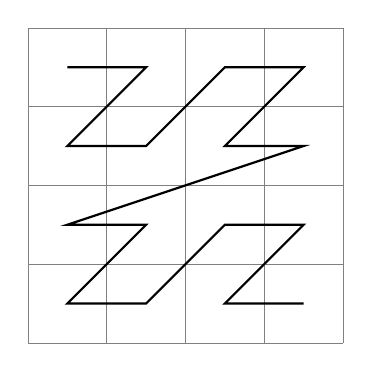
\begin{tikzpicture}
	\draw[step=1cm,gray,very thin] (0,0) grid (4,4);
	% NOTE: TikZ coordinate system has (0,0) in bottom left.
	\draw[thick] (0.5,3.5) -- (1.5,3.5) -- (0.5,2.5) -- (1.5,2.5) --
		(2.5,3.5) -- (3.5,3.5) -- (2.5,2.5) -- (3.5,2.5) --
		(0.5,1.5) -- (1.5,1.5) -- (0.5,0.5) -- (1.5,0.5) --
		(2.5,1.5) -- (3.5,1.5) -- (2.5,0.5) -- (3.5,0.5);
	\end{tikzpicture}
};
\end{tikzpicture}
\caption{Z-order in two dimensions}
\end{figure}

A possible alternative would be using a \emph{Peano curve}
(introduced in \cite{peano-curve}, later generalized into
\emph{Hilbert curves} of arbitrary dimension by \cite{hilbert-curve}).
A desirable property of Peano curves is that points mapped to adjacent
one-dimensional points are also adjacent in the multidimensional space.
We decided to use the Z-order for the simplicity of its mapping function.

Queries are implemented simply by mixed calls to \texttt{dict\_prev} and
\texttt{dict\_next} until we collect enough results. A non-toy database might
perform some additional filtering to ensure only reports within a certain
distance are returned.

Our usage of this simulated database will pick $S$ random points on the globe.
For each point, we fetch $R$ close records and we calculate the average
recorded sea-level atmospheric pressure and wind speed in these records.
Atmospheric pressures and wind speeds are packed into 64-bit values, which
are stored in the ordered dictionary.

\begin{figure}
\centering
\begin{subfigure}[b]{1.0\textwidth}
	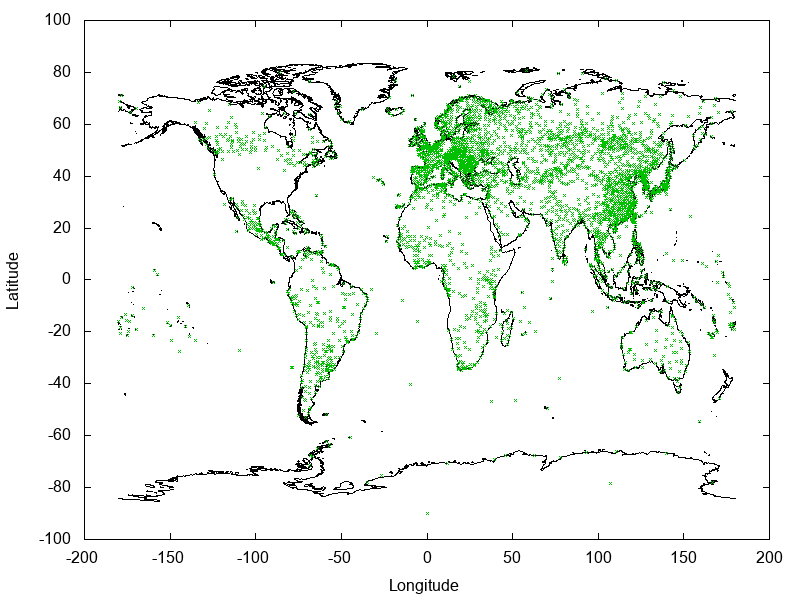
\includegraphics[width=\textwidth]{img/cloud/stations}
	\caption{Stations providing wind speed or air pressure data}
\end{subfigure}

\begin{subfigure}[b]{1.0\textwidth}
	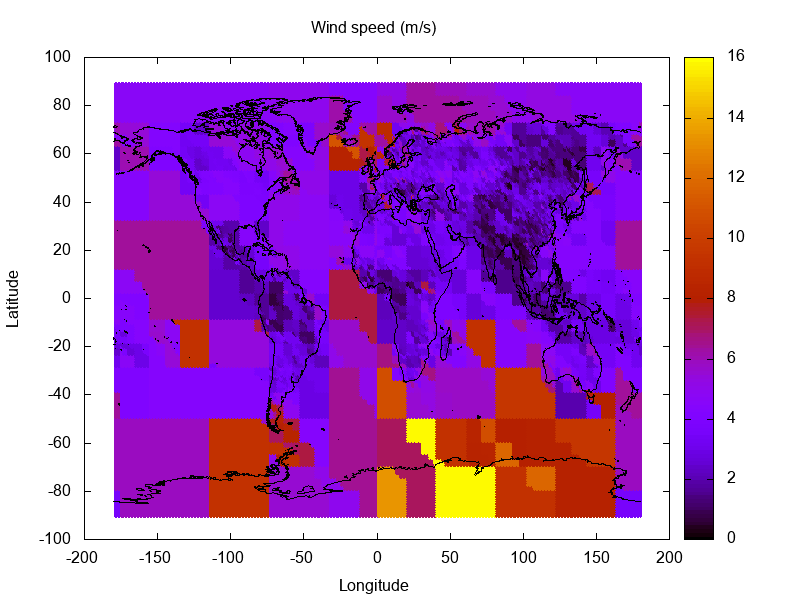
\includegraphics[width=\textwidth]{img/cloud/wind-speed}
	\caption{Average wind speeds}
\end{subfigure}
\end{figure}
\clearpage
\begin{figure}[H]
\centering
\ContinuedFloat
\begin{subfigure}[b]{1.0\textwidth}
	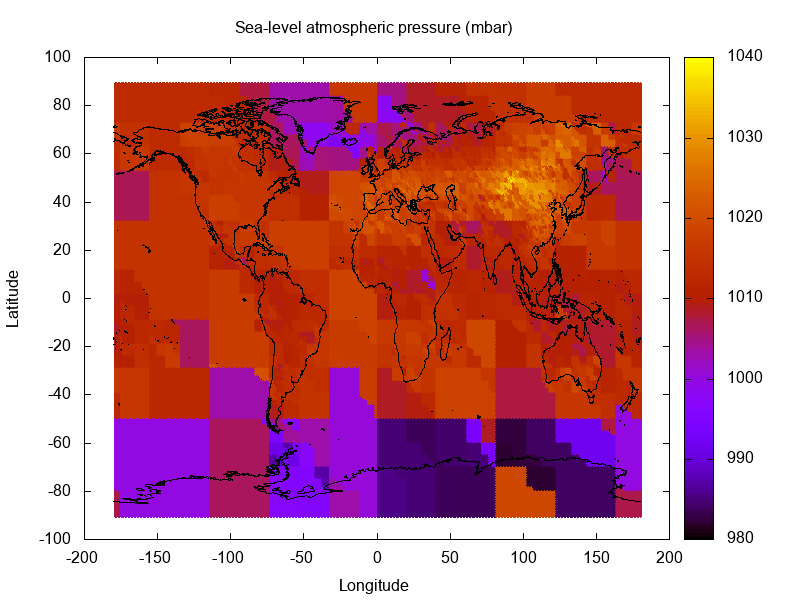
\includegraphics[width=\textwidth]{img/cloud/pressure}
	\caption{Average sea-level atmospheric pressure}
\end{subfigure}
\caption{Results from the cloud data experiment.
	Each query sampled 1000 close measurements.}
\end{figure}
